\section{Auswertung}
\label{sec:Auswertung}
\subsection{Bestimmung der mittleren Weglänge}
In der Tabelle \ref{tab:weglaenge} sind die gemessenen Temperaturen $T$ und der daraus berechnete Sättigungsdruck $p_\text{Sätt}$, die berechnete 
mittlere Weglänge $\overline{w}$ und das Verhältnis aus der mittleren Weglänge und dem Abstand Kathode-Beschleunigungselektrode $a = \SI{1}{\centi\metre}$.
\begin{table}
    \centering
    \caption{Errechnetes Verhältnis der mittleren Weglänge $\overline{w}$ und dem Abstand Kathode-Beschleunigungselektrode $a$}
    \label{tab:weglaenge}
    \begin{tabular} {S[table-format=3.2] S[table-format=2.3] S[table-format=1.3] S[table-format=4.2]}
        \toprule
        {$T \mathbin{/} \si{\kelvin}$} & {$p_\text{Sätt} \mathbin{/} \si{\milli\bar}$} & {$\overline{w} \mathbin{/} \si{\micro\metre}$} 
        & {$\frac{a}{\overline{w}}$}\\
    \midrule
    299.15 & 0.006 & 5062.30 & 2.98\\
    413.15 & 3.254 & 8.91 & 1122.17\\
    438.15 & 8.411 & 3.45 & 2900.48\\
    448.15 & 11.938& 2.43 & 4116.72\\    
    \bottomrule
\end{tabular}
\end{table}
Wie in der Tabelle \ref{tab:weglaenge} zu erkennen ist, liegt nur das Verhältnis bei Raumtemperatur von $\SI{26}{\celsius}$ nicht in dem erforderlichen Bereich von 
1000 bis 4000.
\FloatBarrier
\subsection{Bestimmung des Kontaktpotentials}
In der Tabelle \ref{tab:energie} sind die gemessenen Gegenspannungen $U_\text{A}$ und der Auffängerstrom $I_\text{A}$ bei den Temperaturen 
$T = \SI{26}{\celsius}$ und $T = \SI{140}{\celsius}$ aufgelistet. 
Aus diesen Daten lässt sich der Differenzenquotient 
\begin{equation*}
    \frac{\symup{\Delta}I_\text{A}}{\symup{\Delta}U_\text{A}} = \frac{I_{\text{A}_{i+1}} - I_{\text{A}_i}}{U_{\text{A}_{i+1}} - U_{\text{A}_{i}}}
\end{equation*}
errechnen, 
woraus die in der Abbildung \ref{fig:potentialroom} und \ref{fig:potentialhot} eingezeichnete diskrete differentielle Energieverteilung 
für die Temperaturen $T = \SI{26}{\celsius}$ und $T = \SI{140}{\celsius}$ erstellt werden kann.
Das in der Abbildung eingezeichnete Maximum liegt bei $U_\text{A, max} = \SI{8.5}{\volt}$, woraus sich ein Kontaktpotential von
\begin{equation*}
    K = U_\text{B} - U_\text{A, max} = \SI{11}{\volt} - \SI{8.5}{\volt} = \SI{2.5}{\volt}
\end{equation*}
bestimmen lässt.
\begin{table}
    \centering
    \caption{Gemessen Auffangströme bei $T = \SI{26}{\celsius}$ und $T = \SI{140}{\celsius}$.}
    \label{tab:energie}
    \begin{tabular} {S[table-format=2.0] S[table-format=1.3] S[table-format=2.1] S[table-format=1.1]}
        \toprule
        \multicolumn{2}{c}{$T = \SI{26}{\celsius}$}& \multicolumn{2}{c}{$T = \SI{140}{\celsius}$}\\
        \cmidrule(lr){1-2}\cmidrule(lr){3-4}
        {$U_\text{A} \mathbin{/} \si{\volt}$} & {$I_\text{A} \mathbin{/} \SI{0.01}{\nano\ampere}$} & {$U_\text{A} \mathbin{/} \si{\volt}$} & {$I_\text{A} \mathbin{/} \SI{0.01}{\nano\ampere}$}\\
    \midrule
    0   &  1.8   &   0     &  4.4\\
    1   &  1.75  &   0.5   &  4.2\\
    2   &  1.7   &   1     &  3\\
    3   &  1.6   &   1.5   &  2.6\\
    4   &  1.5   &   2     &  1.6\\
    5   &  1.49  &   2.5   &  1.2\\
    6   &  1.25  &   3     &  0.5\\
    7   &  1     &   3.5   &  0.2\\
    8   &  0.565 &   4     &  0\\
    9   &  0.1   &   5     &  0\\
    10  &  0     &   6     &  0\\
    \bottomrule
\end{tabular}
\end{table}
\begin{figure}
    \centering
    \caption{Differentielle Energieverteilung bei $T = \SI{26}{\celsius}$}
    \label{fig:potentialroom}
    \includegraphics{build/potentialroom.pdf}
\end{figure}
\begin{figure}
    \centering
    \caption{Differentielle Energieverteilung bei $T = \SI{140}{\celsius}$}
    \label{fig:potentialhot}
    \includegraphics{build/potentialhot.pdf}
\end{figure}
\FloatBarrier
\subsection{Bestimmung der Anregungsenergie des $\ce{Hg}$-Atoms}\label{sec:frank}
\begin{table}
    \centering
    \caption{Gemessener Auffängerstrom $I_\text{A}$ in Abhängigkeit von der Beschleunigungsspannung $U_\text{B}$ 
    bei den Temperaturen $T = \SI{165}{\celsius}$ und $T = \SI{175}{\celsius}$.}
    \label{tab:frankherz}
    \begin{tabular} {S[table-format=2.0] S[table-format=1.1] S[table-format=2.0] S[table-format=1.1]}
        \toprule
        \multicolumn{2}{c}{$T = \SI{165}{\celsius}$}& \multicolumn{2}{c}{$T = \SI{175}{\celsius}$}\\
        \cmidrule(lr){1-2}\cmidrule(lr){3-4}
        {$U_\text{B} \mathbin{/} \si{\volt}$} & {$I_\text{A} \mathbin{/} \SI{0.01}{\nano\ampere}$} & {$U_\text{B} \mathbin{/} \si{\volt}$} & {$I_\text{A} \mathbin{/} \SI{0.01}{\nano\ampere}$}\\
    \midrule
    0   &  0    &   0   & 0   \\
    7   &  0.5  &   11  & 0.8\\
    9   &  0    &   14  & 0   \\
    12  &  3    &   15  & 0.6\\
    13  &  1    &   17  & 1.4 \\   
    14  &  0.5  &   19  & 0.1\\
    17  &  5    &   22  & 1.6\\
    18  &  2    &   24  & 0.4\\
    19  &  1.5  &   26  & 1.4\\
    21  &  4    &   30  & 0.6\\
    22  &  5.5  &   33  & 1.2\\
    25  &  3    &   35  & 1   \\
    27  &  6    &   39  & 1.6\\
    30  &  5    &   {-} &{-}\\
    \bottomrule
\end{tabular}
\end{table}
In der Abbildung \ref{fig:frankherz1} und \ref{fig:frankherz2} ist die gemessene Franck-Hertz-Kurve bei $\SI{165}{\celsius}$ bzw. $\SI{175}{\celsius}$ 
graphisch dargestellt.
Die aufgenommenen Messwerte sind verbunden, wodurch die Extrema deutlicher werden sollen.
\begin{figure}
    \centering
    \caption{Frank-Herz-Kurve bei $\SI{165}{\celsius}$}
    \label{fig:frankherz1}
    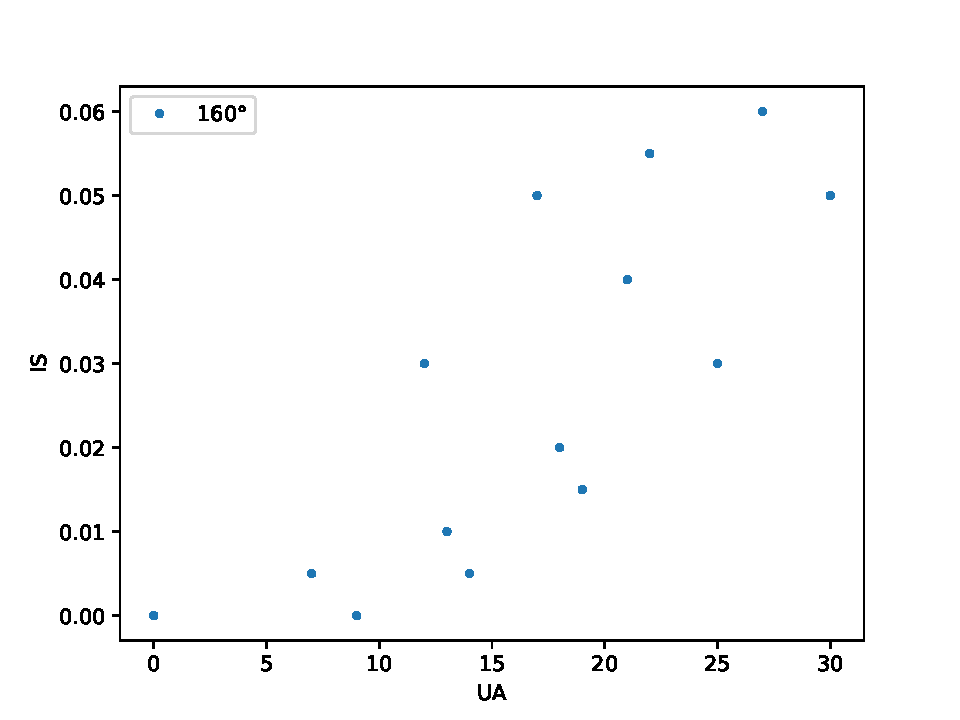
\includegraphics{build/frankherz1.pdf}
\end{figure}
\begin{figure}
    \centering
    \caption{Frank-Herz-Kurve bei $\SI{175}{\celsius}$}
    \label{fig:frankherz2}
    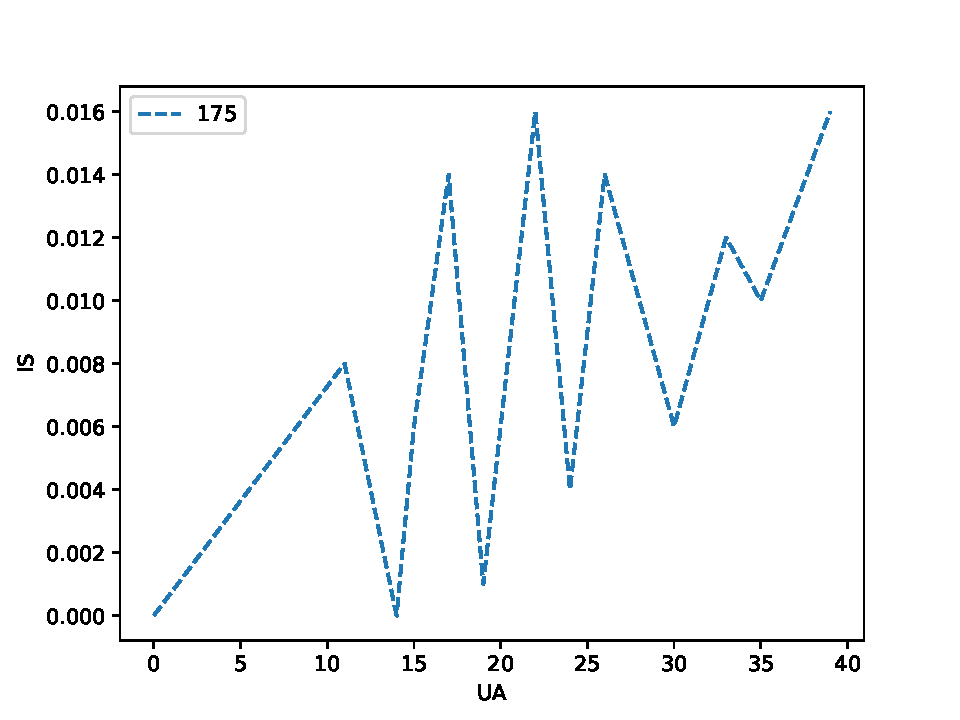
\includegraphics{build/frankherz2.pdf}
\end{figure}
Da die Maxima der Frank-Hertz-Kurve bei $\SI{165}{\celsius}$ stetig größer werden, wird diese zur Bestimmung der Anregungsenergie verwendet.
Die Maxima werden auf dem Intervall $D = [7\si{\volt}, 27\si{\volt}]$ ersichtlich, weswegen die Abstände der Maxima über dieses Intervall gemittelt werden.
Der gemittelte Abstand zwischen den Maxima ergibt sich zu $\bar{U}_\text{1} = \SI{5}{\volt}$.
Daraus kann die Anregungsenergie von dem $\ce{Hg}$-Atom zu 
\begin{equation*}
    E_1 - E_0 = U_1 e_0 = \SI{5}{\electronvolt}
\end{equation*}
bestimmt werden.
Gemäß der Beziehung
\begin{equation*}
    \lambda =  \frac{hc}{E_1 - E_0}
\end{equation*}
lässt sich mit $c = \SI{299792458}{\metre\per\second}$\cite{speedoflight} und $h = \SI{6.62607015e-34}{\joule\second}$\cite{plank}
die Wellenlänge der emittierten Photonen zu
\begin{equation*}
    \lambda = \SI{247.99}{\nano\metre}
\end{equation*}
bestimmen, welche im UV-Bereich liegt.